\section{Introduction}\label{sec:intro}

\noindent Hominin endocranial volume roughly tripled across the Plio-Pleistocene, mostly through change within lineages
rather than species turnover~\cite{puschel2024,du2018}. The increase departed from the brain--body scaling of other
primates~\cite{miller2019}, and it was paid for: a child's brain takes about two-thirds of resting metabolism at its
peak~\cite{kuzawa2014}, and human energy budgets exceed those of other apes~\cite{pontzer2016}. Per generation, however, the
change was slow, about $10^{-4}$ standard deviations~\cite{gingerich2022}. Selection that weak is easy to supply. The puzzle
is persistence: why a costly organ kept its direction for some hundred thousand generations, in several lineages, yet not
in all.

One candidate begins with a problem of timing. Much of what a human partner is worth cannot be seen when partners are
chosen. A forager's hunting skill peaks near age 33~\cite{koster2020,gurven2006}, and the number of children a person
raises is not known until middle age, yet marriages are made in the teens and twenties. A capacity that pays at forty and
cannot be seen at twenty is invisible to any selection that works through other people's choices. Humans fill the gap with
performance: foraging, craft, contest, play and speech, repeated in public for years before lifetime outcomes are known.
If prospective partners, their kin and allies used that evidence, and if their decisions changed who reproduced,
information became selection. Nothing in this requires that a bride chose freely; in most recorded societies she did not
(Section~\ref{sec:reschoice}). It requires that whoever decided had watched for years. The idea has a long history in theories of sexual and social
selection~\cite{miller2000ch,miller2000book,hooper2008,westeberhard1983,nesse2007,flinn2005,crespi2022,progovac2026}, and
animal breeders know its logic as a formula: gain per generation equals genetic variation times the accuracy of selection
decisions times their intensity~\cite{lush1937,hazel1943,falconer1996}. Gain rises sharply when accuracy is obtained
early; genomic prediction at birth raised annual gain in dairy cattle by 50--100\%~\cite{garciaruiz2016}. We call the
hypothesis \emph{performance before outcomes}.

The usual test asks whether intelligence is attractive. That question is too coarse to answer, because selection through
mating is a chain of separable links: \emph{who assesses} (a partner, the partner's kin, rivals, allies); \emph{what they
observe} (a cue, a performance, or a record); \emph{how accurately} it forecasts a heritable capacity; \emph{which episode
of reproduction} the decision governs; and \emph{with what aim}, that is, which trait the observation loads on. We take the
chain apart, state each link as a model with proofs and simulation checks, and measure the links that can be measured: in
the fossil record, in a speed-dating experiment, in a national survey followed for fifty years, in the coded ethnographic
record of \CcSccsN{} societies, and in two cross-national surveys of 45 and 175 countries.

Eight results follow. One observer cannot read a mind and a camp can, and people act only on what they can read. Being
judged across many domains aims selection at the generalist. Capacity is selected only where it is delivered, and delivery
cannot be read from a test that the person recognizes: it has to be observed unannounced or enforced by others. The sexes
are selected at different episodes, then and now: men at the door, women after it. The chooser was seldom a free young
woman: parents and elders decide most marriages in the ethnographic record, coercion is common, and the mechanism needs a
jury with years of evidence, not romance or consent. Culture changes the weights on each link without changing the links.
Where a dangerous test is banned a safe, repeatable one takes its place, and keeps what it showed about capacity while
losing what it showed about nerve. And the jury is now being dismissed: Americans want as many children as they did fifty
years ago, and almost all of the shortfall arises before a couple forms. None of this estimates an ancestral parameter.
The paper derives what would have to be true if mate selection contributed to brain expansion, shows which parts hold in
living people, and lists the observations that would count against it. Proofs, simulations, the evidence base and audits
of common claims are in the Supplementary Information (SI).

\section{Results}

\subsection{A slow, persistent, stepwise expansion}\label{sec:resfossil}

We reanalyzed \FosN{} dated crania~\cite{gingerich2022}. Log volume rose by \FosSlopeSpec{} per million years, which is
\FosRateLo--\FosRateHi{}$\times10^{-4}$ standard deviations per generation. A constant trend fits poorly
($\Delta\mathrm{AICc}=\FosAICLin$). The record is better described by stasis broken by two steps, with change points near
\FosBpA, \FosBpB{} and \FosBpC{} million years ago and plateaus at \FosLevI{} and \FosLevIII\ccm{} (Figs.~\ref{fig:main}A
and~\ref{fig:fossils}A), although analyses of cranial shape favor random walks and stasis~\cite{hubbe2026} and stasis
cannot be told from slow change within phases. Over the last 0.9 million years volume rose in three regional series
(Fig.~\ref{fig:fossils}B): by \SerAfr{} log units per million years in the African series leading to \Hs, \SerEur{} in
western Eurasia leading to Neanderthals, and \SerAsia{} in eastern Asia~\cite{will2021}. Neanderthals (\NeaMean\ccm) were
close to contemporaneous \Hs{} (\SapMean\ccm), while two late species kept brains under 600\ccm, the size of an
australopith's, long after the last australopiths had gone: \textit{H.~naledi} in southern Africa about 0.3 million years
ago~\cite{dirks2017}, and \textit{H.~floresiensis} on the island of Flores until some 60,000 years
ago~\cite{sutikna2016} (Fig.~\ref{fig:fossils}C). They lived at the same time as large-brained people, not beside
australopiths and, on Flores, beside no one: the island was reached only by sea, and the lineage was there by 0.7 million
years ago~\cite{brumm2016,vandenbergh2016}. Volume in our own species has not risen for at least 100,000 years, and recent
populations average \RecentDrop\% less than Pleistocene ones~\cite{beals1984}.

What needs explaining is therefore not speed. If the whole increase were a correlated response to selection on a cognitive
capacity, the selection differential required is about $\ReqBase$ standard deviations per generation
(Section~\ref{sec:strength}). The questions are why the direction persisted, why benefits kept pace with rising cost, why
several lineages moved in parallel while others did not, and why change came in steps.

\begin{figure*}[t]
\centering
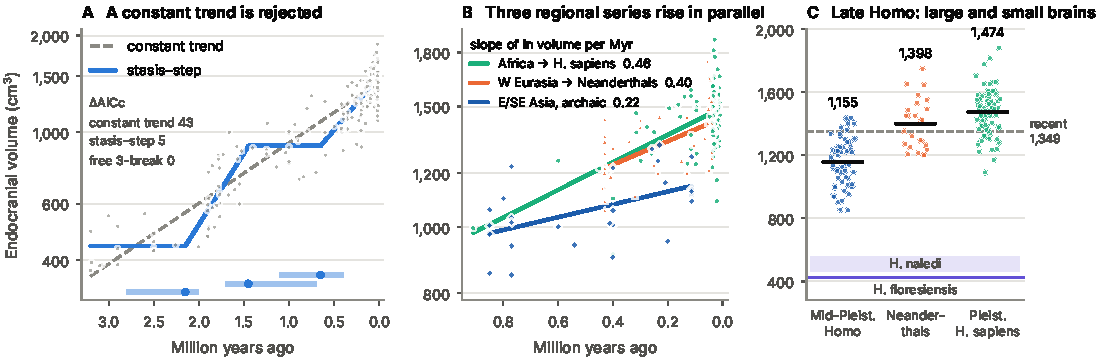
\includegraphics[width=\textwidth]{figures/fig2_fossils.pdf}
\caption{\textbf{The fossil record: slow, stepwise, parallel.} \textbf{(A)}~Endocranial volume of \FosN{} crania~\cite{gingerich2022}
with a constant trend and the stasis--step model; bars at the bottom are bootstrap 95\% intervals for the change points.
\textbf{(B)}~Three regional series over the last 0.9~Myr with fitted slopes~\cite{will2021}. \textbf{(C)}~Late \Homo: specimens and
group means for Middle Pleistocene \Homo, Neanderthals and Pleistocene \Hs~\cite{will2021}; bands mark
\textit{H.~naledi} and \textit{H.~floresiensis}~\cite{berger2015,kubo2013}; the dashed line is the mean of recent
populations~\cite{beals1984}. Claim level: reanalysis of published open data.}
\label{fig:fossils}
\end{figure*}

\subsection{Mate selection has five links}\label{sec:decomp}

The breeder's equation organizes the first three links. If decisions rest on a score $Y$ whose squared correlation with a
capacity is the validity $R$, the response of the capacity's breeding value per generation is
\begin{equation}
S=\sigma_A\cdot h\sqrt R\cdot i,\qquad i=\Corr(Y,W)\,\CV(W),\label{eq:mainidentity}
\end{equation}
genetic standard deviation times accuracy times intensity, where $W$ is reproductive contribution
(Proposition~\ref{prop:identity}). Information enters as $\sqrt R$, so poor information still has an effect, and it is
separable from reproductive inequality: validity can change the response while the distribution of reproduction stays fixed.
\emph{Who assesses} and \emph{what they observe} set $R$. A static cue is read at a glance; a performance has an outcome and
can be repeated; a record accumulates many performances and travels by talk. Parents arrange most marriages in foraging
societies~\cite{walker2011,apostolou2007} and weigh a suitor's investment and cooperation more than their children
do~\cite{buunk2008}; a model with only the partner's choice mistakes one juror for the jury.

The fourth link is the episode. Lifetime reproduction is a sequence, and a selection differential is the sum of the
contributions of its stages~\cite{arnold1984}. For a standardized trait $z$ and completed family size $c$ the split is exact
(Proposition~\ref{prop:episodes}):
\begin{equation}
S=\underbrace{\E[z\mid c>0]}_{\text{access}}+\underbrace{\frac{\Cov(z,c\mid c>0)}{\E[c\mid c>0]}}_{\text{number}}.\label{eq:split}
\end{equation}
Access, becoming a parent at all, is decided largely by other people, though intention, infertility and timing enter it
too. It divides further into pairing and the conversion of a partnership into parenthood. Number depends on timing and on
the stability of unions. Under natural fertility a third term, the survival of children, is at least as
large~\cite{volk2013,sear2008}. Table~\ref{tab:anatomy} sets out the links by sex.

The fifth link is aim. A score loads on some traits more than others, and the loading, not the intensity of competition,
decides what evolves.

\begin{table*}[t]
\caption{The anatomy of mate selection by episode and sex. ``Small-scale societies'' summarizes cited field evidence
(Sections~\ref{sec:evidence} and~\ref{sec:hidden}); ``today'' summarizes Section~\ref{sec:restoday}. Entries describe where trait
variation is converted into reproductive variation; none is an estimate of ancestral selection.}
\label{tab:anatomy}
\scriptsize
\begin{tabularx}{\textwidth}{@{}P{0.115\textwidth}P{0.125\textwidth}LLP{0.205\textwidth}@{}}
\toprule
Episode & Decided mainly by & What varies among men & What varies among women & Today (United States, this paper)\\
\midrule
Access: obtaining a partner and becoming a parent &
Prospective partner; the partner's parents and kin; rivals and allies &
Large. Men's standing predicts reproductive success across 33 societies~\cite{vonrueden2016}; kin arrange most marriages and
apply their own criteria~\cite{walker2011,apostolou2007,apostolou2010}; men's variance in reproductive success usually exceeds
women's~\cite{brown2009,betzig2012}. &
Smaller. Assessed qualities affect \emph{whom} a woman marries (partner quality) more than whether she does; Hadza men
look for hard work and women for intelligence and foraging skill~\cite{marlowe2004}. &
Men: income and standing favored at pairing; childlessness concentrated at the bottom of the income distribution. Women: no
effect at pairing over the whole period; schooling, standing and income lower the chance of motherhood
(Tables~\ref{tab:gss} and~\ref{tab:funnel}).\\
\addlinespace
Timing: age at first birth &
The couple and their kin &
Prestigious Tsimane men marry wives who first give birth at younger ages, the strongest path from status to fitness
there~\cite{vonrueden2011}. &
Earlier first birth lengthens the reproductive span. &
Later first birth, which goes with more schooling, accounts for \GssTimShareW\% (women) and \GssTimShareM\% (men) of the
schooling--family-size relation among parents.\\
\addlinespace
Number: births while partnered; remarriage, polygyny &
The couple; rivals for additional partners &
Serial marriage raised men's number in the United States and polygyny did in nineteenth-century
Utah~\cite{jokela2010,moorad2011}. Among Pimbwe, once years married are held constant, extra partners help women and not
men~\cite{borgerhoffmulder2019}. &
Birth spacing, limited by energy and help. Extra husbands added little in the United States and Utah
samples~\cite{jokela2010,moorad2011}. &
Negative association with schooling, vocabulary and standing in both sexes; a second marriage adds children for men
only; more sexual partners go with fewer children.\\
\addlinespace
Survival of off\-spring &
The mother; allomothers; the father's provisioning &
Provisioning and protection. Prestigious Tsimane men have lower offspring mortality~\cite{vonrueden2011}; which relatives
improve child survival varies among societies~\cite{sear2008}. &
Large. A mother's knowledge~\cite{mcdade2007}, standing~\cite{alami2020} and kin help~\cite{sear2008} predict child health and
survival. &
Negligible variance: nearly all children survive.\\
\bottomrule
\end{tabularx}
\end{table*}

\emph{The assessor need not be the bride, and the choice need not be free.} The identity holds for any assessor. If a
share $\kappa$ of matings is settled without regard to the assessed trait, by capture or coercion, the differential on
that trait is
\begin{equation}
S=(1-\kappa)\,S_{\text{assessed}}+\kappa\,S_{\text{force}},\label{eq:coercion}
\end{equation}
where $S_{\text{force}}$ is whatever a contest of force selects, which is the body (Section~\ref{sec:rescontest}).
Coercion subtracts from the pathway in proportion to its share and puts selection on formidability in its place
(simulation: largest error \NtCoeErr). Section~\ref{sec:reschoice} reports what the ethnographic record codes about who
the assessor was and about $\kappa$.

\subsection{One observer cannot read a mind; a camp can}\label{sec:resjury}

How much does one meeting reveal, and how fast do observers converge? In the Columbia speed-dating
experiment~\cite{fisman2006}, \SdN{} graduate students met in \SdSessions{} sessions; each pair talked for four minutes,
rated the other on six attributes and said yes or no to meeting again (\SdRows{} meetings; Methods). Two observers of the
same person agree \JurOneAtt{} about looks and \JurOneFun{} about how much fun someone is, but only \JurOneInt,
\JurOneAmb{} and \JurOneSin{} about intelligence, ambition and sincerity. Agreement between two panels of $k$ observers
then rises as the Spearman--Brown law requires~\cite{spearman1910,brown1910},
\begin{equation}
r_k=\frac{k\,r_1}{1+(k-1)\,r_1},\label{eq:sb}
\end{equation}
to within \JurGapMax{} at every panel size we could test (Fig.~\ref{fig:main}B). A dependable verdict ($r_k=0.8$) takes
\JurKAtt{} observers for looks, \JurKFun{} for fun, \JurKInt{} for intelligence and \JurKSin{} for sincerity. A suitor
cannot read a mind in an evening. A camp of a few dozen people~\cite{hill2011} that has watched someone for years can.
The gain comes only from independent observation. If observers share a fraction $c$ of their error, as people repeating
one report do, their consensus grows while its accuracy cannot exceed $r_1/[r_1+c(1-r_1)]$: \JurCeil{} for a trait read as
poorly as intelligence, at $c=0.3$ (Section~\ref{sec:speed}).
Asking does not help: self-ratings of intelligence and sincerity correlate \SdSelfInt{} and \SdSelfSin{} with the panel's
verdict. Nor is the verdict mere consensus: the panel's rating of intelligence, and not of looks, tracks the median
entrance-test score of the person's college ($r=\SdSat$; \SdSatCI; $n=\SdSatN$).

\emph{People act on what they can read.} Before the event women gave most weight to intelligence and sincerity, and men to
looks and then intelligence. What earned a yes was looks above all, in both sexes, then shared interests and fun;
intelligence earned little, sincerity and ambition nothing (Fig.~\ref{fig:jury}A). The sexes differ less in what they do
than in what they say~\cite{eastwick2014,eastwick2025}: men respond more to looks (by \SdRevDiffAtt{} points per standard
deviation; \SdRevDiffAttCI) and women slightly more to intelligence (\SdRevDiffInt; \SdRevDiffIntCI), as the original
authors found~\cite{fisman2006}, but the profiles have one shape. That shape is the order in which four minutes can read
the attributes ($r=\SdLegPear$ between agreement and effect across the five personal attributes; Fig.~\ref{fig:jury}B).
With five attributes this cannot separate legibility from taste (prediction P27), but it is what the theory requires: a
preference is only as strong as the instrument that serves it. Societies that select on mind and character must possess
instruments that read them.

\emph{Access is unequal within minutes, and misjudged.} Women said yes to \SdYesW\% of partners and men to \SdYesM\%;
\SdPopZeroM\% of men and \SdPopZeroW\% of women received no yes at all. Each sex expected a yes from \SdExpW\% of partners.
Women received one from \SdActW\% and men from \SdActM\%: men overestimated their welcome by \SdGapM{} points (\SdGapMCI)
and women did not (Fig.~\ref{fig:jury}C), the asymmetry that error-management theory
predicts~\cite{haselton2000,perilloux2012}. Neither sex knew which partners had said yes (correlations of \SdAccM{} and
\SdAccW{} between guess and outcome).

\begin{figure*}[t]
\centering
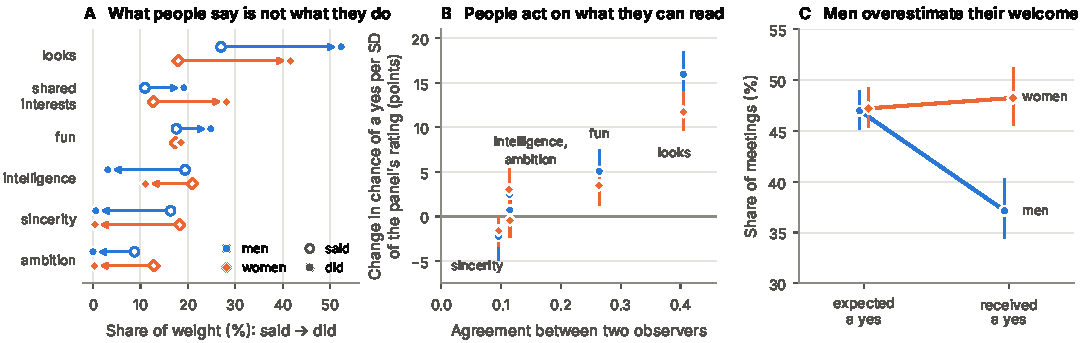
\includegraphics[width=\textwidth]{figures/fig3_jury.pdf}
\caption{\textbf{Said, done, and what four minutes can read.} Columbia speed-dating experiment~\cite{fisman2006}: \SdN{}
people, \SdRows{} meetings; men are circles and women diamonds; whiskers are 95\% bootstrap intervals. \textbf{(A)}~For each
attribute, the share of 100 points given to it before the event (open markers) and its share of the summed positive
effects on a yes (filled markers); arrows run from said to did. \textbf{(B)}~Change in the probability of a yes per standard
deviation of everyone else's rating of the partner, against the agreement between two observers of the same person.
\textbf{(C)}~Share of meetings in which a person expected a yes (the 1--10 guess rescaled to 0--100) and in which a yes was
received. Claim level: reanalysis of public data.}
\label{fig:jury}
\end{figure*}

\emph{Night talk and long acquaintance.} Published results show the same thing outside the laboratory. Among 167
couples, those who had known each other longer before dating were less alike in rated attractiveness: agreement about who
is desirable is strongest early in acquaintance and gives way as people learn what a glance cannot
show~\cite{hunt2015}. Two-thirds of adults in seven samples said their romance began as a
friendship~\cite{stinson2022}. The forager's instrument for this was the evening. Among the Ju/'hoansi, talk by day was
of practical matters and complaints about others, and talk by firelight was stories~\cite{wiessner2014}; people in three
societies without electricity fall asleep 3.3 hours after sunset on average~\cite{yetish2015}. Fire lengthened the day
for observation as well as for digestion~\cite{dunbar2014}. It added occasions, an audience, and a domain, speech, on
which everyone present could be compared. The payoffs are measurable in living foragers: skilled Agta storytellers are
preferred as camp-mates and have more surviving children~\cite{smith2017}; Agta and BaYaka mothers who are better
connected in the camp's network of contacts have more living offspring~\cite{page2017}; and BaYaka with more partners in
cooperation are better nourished, the women more fertile~\cite{chaudhary2016}.

\subsection{Breadth aims selection at the generalist}\label{sec:resgeneralist}

Let performance in each of $K$ domains be the sum of a general capacity $G$ and a domain-specific one, and let standing
depend on the average across domains. Then the selection differential on general capacity relative to that on any one
specialty is
\begin{equation}
\frac{S_{A_G}}{S_{A_{S_k}}}=K\,\frac{V_{A,G}}{V_{A,S}}\label{eq:mainaim}
\end{equation}
(Corollary~\ref{cor:generalist}; Fig.~\ref{fig:main}C). One venue cannot tell a generalist from a specialist. Each added venue
dilutes every specialty and leaves the pull on what the venues share undiminished. Four further results sharpen this.

\emph{Breadth buys time.} With few domains, no amount of watching reaches a given accuracy for general capacity, because
domain-specific ability and persistent error never average out; with many, a little evidence from each suffices
(Proposition~\ref{prop:time}; Fig.~\ref{fig:polymath}A). Mastery of any one demanding skill arrives late, so a specialist's
quality is known late. A generalist's can be known early, from how a young person does in many things, including how
quickly new ones are picked up. Performance before outcomes is feasible for general capacity in a way that it is not for a
single skill.

\emph{Expenditure follows breadth.} If general capacity costs $c_G$ per unit and specific skill $c_S$, the share of
investment devoted to general capacity at equilibrium is $Kc_S/(Kc_S+c_G)$, which passes one half when the number of commonly
assessed domains equals the cost ratio (Proposition~\ref{prop:polymath}; Fig.~\ref{fig:polymath}B). General capacity is the
expensive kind if it resides in tissue serving every domain, so a lineage with a narrow repertoire should invest in
specialized skill however intense its competition, and one with a broad repertoire in general capacity. Cumulative culture
adds domains, which ties the demand for a general-purpose brain to the breadth of culture and not to its depth.

\emph{Breadth taxes show.} Inflating one performance moves a $K$-domain average by $1/K$ of the inflation, while general
capacity moves it in full, so common comparison dilutes exaggeration exactly as it dilutes specialty, without requiring
that display be costly (Corollary~\ref{cor:inflation}; Fig.~\ref{fig:polymath}C). What it cannot dilute is a talent for
seeming that carries across every venue.

\emph{Division of labor restores the specialist.} If each person performs, and is compared, only in the domain of their
greatest talent, the aim on general capacity weakens by a factor $Kc_K$, where $c_K$ is the variance of the largest of $K$
standard normal variables: \PolyDivFive-fold for five domains and \PolyDivTen-fold for ten (Proposition~\ref{prop:division};
grey line in Fig.~\ref{fig:main}C). What removes the generalist aim is the loss of a common set of domains, not esteem for
excellence.

The conditions for the generalist aim were met in small societies without occupational specialization. Tsimane adults
command a broad repertoire across food production, child care, craft, music and storytelling, most of it before first
reproduction~\cite{schniter2015}. The general factor has biological standing: across 62 primate species, innovation,
social learning, tool use and extractive foraging form one composite that covaries with brain volume~\cite{reader2011}; most
genetic influences on human cognitive abilities are shared across abilities~\cite{kovas2006,plomin2015}; and the cortex that
expanded most in our lineage is association cortex~\cite{hill2010,buckner2013}, recruited by demanding tasks of every
kind~\cite{duncan2010}. Two cautions apply. A portfolio rewards whatever is common to all venues, which includes health,
condition and opportunity as well as cognition. And the argument shows what such selection would favor, not that it
occurred.

\begin{figure*}[t]
\centering
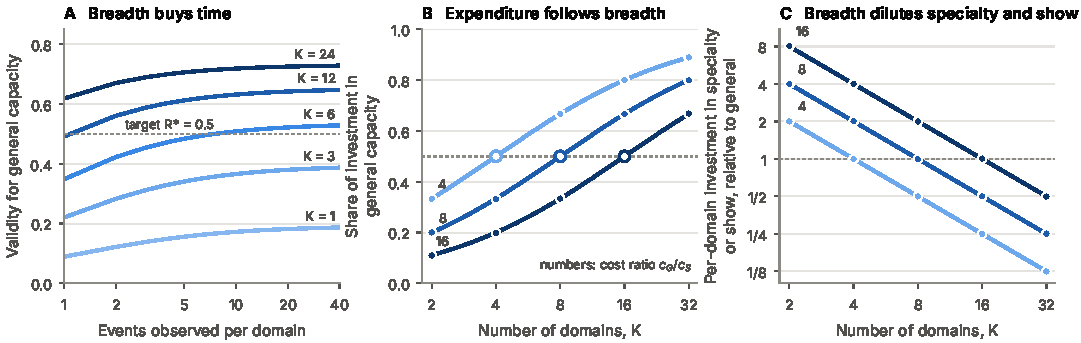
\includegraphics[width=\textwidth]{figures/fig4_polymath.pdf}
\caption{\textbf{Selecting the generalist.} \textbf{(A)}~Breadth buys time: validity for general capacity against events observed
per domain, for 1 to 24 domains (Eq.~\ref{eq:RG}); the dashed line is the target $R^*=0.5$, reached only with more than
five domains (Proposition~\ref{prop:time}). \textbf{(B)}~Expenditure follows breadth: share of investment cost devoted to general
capacity at evolutionary equilibrium, for three ratios of the cost of general to specific capacity; curves are
Eq.~\eqref{eq:share}, markers individual-based simulations, and open circles mark the threshold $K^\dagger=c_G/c_S$.
\textbf{(C)}~Breadth dilutes specialty and show: equilibrium investment per domain in a specific skill, or in exaggerating one
performance at the same cost, relative to investment in general capacity (lines: Eq.~\ref{eq:gstar}; markers: the same
simulations). Parameters are illustrative (Table~\ref{tab:experiments}). Claim level: exact results with numerical checks.}
\label{fig:polymath}
\end{figure*}

\subsection{Contests of force select the body}\label{sec:rescontest}

Popular accounts give fighting the leading role. A contest of force loads on formidability. In the model, moving the basis
of standing from dominance to prestige raises selection on general capacity \AimGain-fold and lowers selection on
formidability \AimLoss-fold at the same intensity (Proposition~\ref{prop:aim}). The comparative record agrees: across primates,
stronger male contest goes with dimorphism in body and canine size~\cite{plavcan2012} and not with larger
brains~\cite{schillaci2006,lemaitre2009,fitzpatrick2012}. Contest contributed to the mind indirectly. Restraint makes contests
repeatable, and repetition is information: validity rises from \RepROne{} for a single decisive fight toward \RepRsafe{} when
bouts are cheap enough to hold nineteen (Proposition~\ref{prop:repeat}). And strong rival coalitions make it rational even for
a dominant to share reproduction (Proposition~\ref{prop:despot}), which lowers intensity \DesIntLo- to \DesIntHi-fold while
moving the criterion of standing from force toward esteem conferred by others~\cite{boehm1993,wrangham2018}. Leveling slows
selection and re-aims it.

\emph{When a dangerous test is banned, a safe one takes its place.} Games with a winner and a loser are recorded in
\CcGamesAny{} of \CcGamesN{} societies with data~\cite{roberts1959,kirby2016}. Men who take part in Sereer ritual
wrestling have more children, although women rank wrestling low among the qualities they say they
want~\cite{llaurens2009}: the verdict of a public contest is used by someone other than the bride. A current case shows
the substitution as it happens. A Maasai warrior once proved himself by killing a lion. With lions scarce and the hunt
illegal, elders conceived in 2008, and first held in 2012, a tournament of running, throwing and a standing high jump
modeled on the warriors' jumping dance, to stand in for the hunt as the mark of manhood, bravery and
prestige~\cite{maasaiolympics,aljazeera2022,hazzah2009,goldman2013}. A man may by custom marry only after the ceremony
that ends warriorhood~\cite{aljazeera2023,spencer1988}; we found no source that makes the height of a jump a condition of
marriage, and standing, not eligibility, is what the jump confers. The theory says what such a change keeps and what it
loses. For capacity it loses nothing: $n$ repetitions of a safe trial of reliability $\rho_s$ match one dangerous trial
of reliability $\rho_d$ once
\begin{equation}
n\ \ge\ \frac{\rho_d\,(1-\rho_s)}{\rho_s\,(1-\rho_d)}\label{eq:ritual}
\end{equation}
(Corollary~\ref{cor:ritual}), which is \NtRitA{} jumps when one jump tells a fifth as much as the hunt, and the whole
community can watch each of them. For willingness to face real danger it loses everything, because a tournament is a
recognized test (Section~\ref{sec:resverify}). That has to be read elsewhere, in years of herding and of service to the
age-set. Safe, repeatable rituals are how a society keeps reading capacity when it can no longer afford the price of the
old test.

\subsection{Capacity is selected only where it is delivered}\label{sec:resdelivery}

A partner's capacity is worth nothing to a chooser unless its product arrives. Let $b$ be the benefit a candidate can
produce and $p$ the share that reaches the chooser and the chooser's children. With value $pb$, the selection differentials
on the two traits are $S_{A_B}\propto\bar p\,R_b$ and $S_{A_P}\propto\bar b\,R_p$ (Proposition~\ref{prop:delivery}). Where
partners deliver nothing, choice for benefits puts no selection on capacity, however able the candidates. The two traits
are complements, so capacity and commitment rise together or not at all, and the take-off has a threshold. And the two
are known through different evidence: capacity shows in performance, which is public and quick; delivery shows in conduct
when interests conflict, which is private and slow.

Present-day evidence fits the distinction. Warmth and trustworthiness form a factor of partner ideals separate from
attractiveness and from status~\cite{fletcher1999}; kindness behaves as a necessity in both sexes~\cite{li2002}; a partner's
perceived commitment and appreciation predict the quality of a relationship where the partner's traits add
nothing~\cite{joel2020}; responsiveness raises desire~\cite{birnbaum2016}; and about two-thirds of relationships in seven
samples began as friendships~\cite{stinson2022}. Human paternal investment, unusual among
mammals~\cite{geary2000,marlowe2000}, is what makes $\bar p$ large enough for the rest of the mechanism to matter.

\subsection{A test shows what a person can do, not what the person will do}\label{sec:resverify}

A candidate who knows when assessment is taking place can change what it shows, and capacity and delivery respond in
opposite ways. Capacity cannot be displayed beyond its level, so the occasions on which a person tries hardest are the best
evidence of it. Delivery is a choice, so an occasion known to be a test says nothing about what will be chosen later. If a
share $d$ of $n$ observed occasions is recognizable as assessment, the validities for capacity and delivery are
\begin{equation}
R_b=\frac{V_B}{V_B+\sigma^2/(dn)},\qquad R_p=\frac{V_P}{V_P+\nu/[(1-d)n]}\label{eq:mainstaging}
\end{equation}
(Proposition~\ref{prop:staging}; Fig.~\ref{fig:main}D). Only occasions that cannot be told from ordinary life inform an
assessor about delivery, and after $m$ of them without a default the default rate is bounded only by about $3/m$:
reliability is never established, only not yet refuted. The speed-dating data show the limit case. A four-minute date is
all test, and sincerity is the attribute it reads worst and rewards least (Fig.~\ref{fig:jury}B). People reason as the
result requires. They ask first whether another person intends good or ill and then whether that person can act on the
intention~\cite{fiske2007}; they weigh good performances more heavily in judging competence and bad conduct more heavily in
judging character~\cite{reeder1979,wojciszke1993}; and maximum and typical performance correlate only
moderately~\cite{beus2012}. Display also bends toward its audience: single women in a business school reported lower
desired salaries and less willingness to travel when single male classmates would see their answers, and no less when the
answers were private~\cite{bursztyn2017}. The practices that add unstaged observation are familiar: long acquaintance
before commitment~\cite{wachtmeister1999,seymour2009,stinson2022}, brideservice under the eyes of
in-laws~\cite{walker2011}, life in a group small enough that conduct is seen daily, and reports from people whose
interests differ from the candidate's.

The alternative to verifying a disposition is to make it matter less. If third parties enforce delivery of a share $e$ of
every candidate's product, as foragers' norms of sharing do~\cite{woodburn1982,peterson1993,wiessner2005}, capacity is
selected in proportion to $e+(1-e)\bar p$ and commitment in proportion to $1-e$ (Proposition~\ref{prop:enforce}).
Enforcement therefore removes the take-off threshold: capacity is selected from the outset, with no evolved commitment at
all (Fig.~\ref{fig:verify}A). It also hides disposition from selection, so evolved commitment is greatest under partial
enforcement, and where choice alone would have sufficed, enforcement crowds commitment out and can lower what is
delivered in all (Fig.~\ref{fig:verify}B). On this reading leveling did more than change the criterion of standing
(Section~\ref{sec:rescontest}): by enforcing delivery it made capacity worth choosing before commitment had evolved. As
history that order is conjecture.

\begin{figure*}[t]
\centering
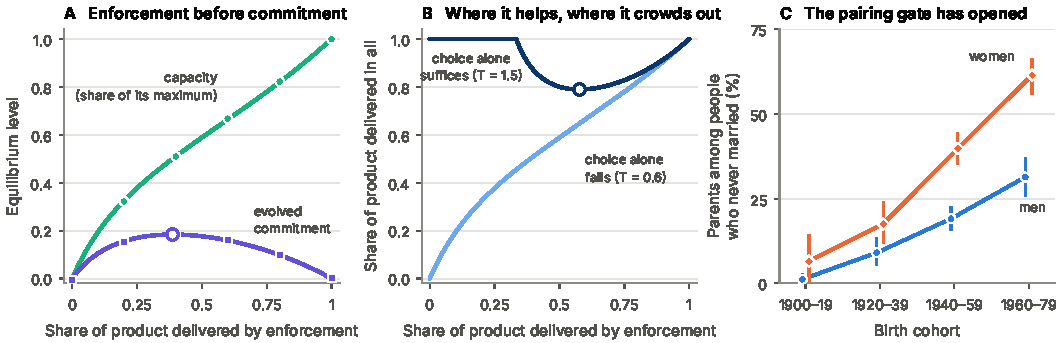
\includegraphics[width=\textwidth]{figures/fig5_verify.pdf}
\caption{\textbf{Enforcement, and a gate.} \textbf{(A)}~Equilibrium capacity, as a share of its maximum, and evolved commitment
against the share of product whose delivery third parties enforce, when choice alone is below the take-off threshold
($T=\EnfT$; Proposition~\ref{prop:enforce}); lines: exact; markers: individual-based simulation; the open circle marks the
peak of commitment. \textbf{(B)}~Share of product delivered in all, enforced plus volunteered, below the threshold ($T=\EnfT$)
and above it ($T=\EnfCrowdT$), where enforcement lowers delivery to a minimum of \EnfCrowdMin{} (open circle).
\textbf{(C)}~Among people who never married, the percentage who are parents, by birth cohort and sex, United States General
Social Survey, ages 45--79; whiskers are 95\% bootstrap intervals; men are circles and women diamonds. Parameters in A and
B are illustrative (Table~\ref{tab:experiments}). Claim level: A and B, exact results with numerical checks; C, reanalysis
of public data~\cite{gss2024}.}
\label{fig:verify}
\end{figure*}

\subsection{Men are selected at the door, women after it}\label{sec:ressexes}

In small-scale and historical societies the episode differs by sex (Table~\ref{tab:anatomy}). For men it is access. Men's
standing predicts reproductive success across 33 societies~\cite{vonrueden2016}; men's variance in reproductive success
usually exceeds women's~\cite{brown2009,betzig2012}; and in a Finnish population with every episode recorded, variance in mating
success explained most of men's excess variance in fitness~\cite{courtiol2012}. For women it is the survival of children and
the timing of the first birth. A Tsimane mother's plant knowledge predicts her children's health~\cite{mcdade2007}, her
political influence predicts their growth and freedom from illness~\cite{alami2020}, relatives improve child survival in
almost every population studied~\cite{sear2008}, and prestigious men gain chiefly through wives who start
earlier~\cite{vonrueden2011}. Selection on women's competence and social skill did not need anyone's choice of them. Cognition
is nonetheless similar in the two sexes, as shared inheritance guarantees whichever sex is selected~\cite{lande1980}.

\label{sec:restoday}Present-day data cannot show what happened in the Pleistocene, but they show which features of human
mate selection persist when fertility is controlled. We applied Eq.~\eqref{eq:split} to \GssN{} adults aged 45--79 in the
United States General Social Survey~\cite{gss2024}, for four traits standardized within sex and birth decade
(Table~\ref{tab:gss}; Methods).

\emph{Number runs against every trait in both sexes.} Among parents, more schooling, a larger vocabulary, a more
prestigious occupation and a higher income go with fewer children. Later first births account for \GssTimShareW\% of the
relation with schooling among mothers and \GssTimShareM\% among fathers.

\emph{Access has opposite signs in the two sexes.} For income the access component is \GssIncMAcc{} (\GssIncMAccCI) in men and
\GssIncWAcc{} (\GssIncWAccCI) in women. For men the two episodes cancel, leaving a total near zero: what pairing rewards,
family size takes back, and a single correlation between status and fertility would report no selection where there are
two opposed episodes.

\emph{For men the door is marriage, and it is a floor.} Splitting access into pairing (ever marrying) and conversion
(parenthood given pairing) puts all of men's advantage at the first step: \GssIncMPair{} (\GssIncMPairCI) for income at
pairing and \GssIncMConv{} at conversion (Fig.~\ref{fig:main}E; Table~\ref{tab:funnel}). Occupational standing, schooling
and vocabulary are also positive at pairing in men. Childlessness falls from \GssQfMOne\% in the lowest fifth of men's
income to \GssQfMThree\% in the middle fifth and \GssQfMFive\% in the highest (Fig.~\ref{fig:today}A); \GssNmMOne\% of men
in the lowest fifth never married, against \GssNmMFive\% in the highest, and the gradient is concentrated at the bottom
(difference in differences \GssFloorM{} percentage points; \GssFloorMCI). Standing buys a man a marriage, not more partners
and not more children: the rank correlation between a man's income and his lifetime number of sexual partners is
\GssPartIncM{} (\GssPartIncMCI), and family size is highest for people reporting one lifetime partner
(Fig.~\ref{fig:today}C).

\emph{For women the selection comes after the door.} Pooled over cohorts, no trait has a detectable effect on whether a
woman marries (income: \GssIncWPair; \GssIncWPairCI); the negative access component arises at conversion (\GssIncWConv),
and childlessness rises from \GssQfWOne\% to \GssQfWFive\% across fifths of women's income. In women born 1960--1979 the
sign at the door has turned: higher income now goes with marrying (\GssPairWNew; \GssPairWNewCI), while its relation to
motherhood within marriage has grown more negative (\GssConvWNew; \GssConvWNewCI). The same trait is now favored at the
door and disfavored after it.

\emph{Leaving and re-entering a marriage pays men only.} Relative to people of their sex and birth decade in a first
marriage, remarried men have \GssRemM{} more children (\GssRemMCI) and remarried women \GssRemW{} (\GssRemWCI); men who
divorced and did not remarry have \GssDivM{} (\GssDivMCI) and such women \GssDivW{} (Fig.~\ref{fig:today}F), as serial
marriage does elsewhere~\cite{jokela2010}.

\emph{The gate passes less and selects more.} Selection at pairing can act only on reproduction that passes through
pairing. Among people born 1920--1939, \GssGateMOld\% of never-married men and \GssGateWOld\% of never-married women were
parents; among those born 1960--1979 the figures are \GssGateMNew\% and \GssGateWNew\% (Fig.~\ref{fig:verify}C). Over the
same cohorts the share of men never marrying rose from \GssNevMOld\% to \GssNevMNew\% and the pairing differential on
men's income rose from \GssPairMOld{} to \GssPairMNew{} (change \GssPairMChange; \GssPairMChangeCI;
Table~\ref{tab:gssgate}). Who marries whom changed too: wives had more schooling than their husbands in \GssHypMoreMid\% of
marriages of people born 1940--1959 and less in \GssHypLessMid\%; for those born from 1980 the figures are
\GssHypMoreYoung\% and \GssHypLessYoung\%, the reversal seen worldwide~\cite{esteve2016}. Many births outside marriage are
to cohabiting couples~\cite{lundberg2016}, so these figures describe marriage, not partnership. Meanwhile access has
tightened at younger ages: at 22--34 the share with no sexual partner in the past year rose from \GssPlMOld\% to
\GssPlMNew\% among men and from \GssPlWOld\% to \GssPlWNew\% among women between 1989--2002 and 2016--2024, and it is graded
by income in both sexes (Fig.~\ref{fig:today}D; Table~\ref{tab:funnel})~\cite{ueda2020}. Childlessness now carries
\GssShareMNew\% of the opportunity for selection among men and \GssShareWNew\% among women born 1960--1979, up from
\GssShareMOld\% and \GssShareWOld\% in those born 1920--1939 (Fig.~\ref{fig:today}E).

These patterns replicate and extend earlier reports. Low-income men are more often childless in Britain, Sweden, the Nordic
countries and the United States, while the relation for women is negative or
reversing~\cite{nettle2008,fieder2007,barthold2012,hopcroft2021,weeden2006,kolk2023,jalovaara2019,kolk2019}. In the Nordic countries the
negative gradient of women's education has vanished~\cite{jalovaara2019}, so the sign for women tracks institutions; the
positive sign for men is found wherever it has been sought. Genetic evidence points the same way. Scores for educational
attainment are negatively associated with number of children, largely through timing~\cite{kong2017,beauchamp2016,hughjones2022},
and carriers of rare damaging variants are more often childless, men especially, apparently for want of a
partner~\cite{gardner2022}. The differentials here are phenotypic, from one country, and self-reported; income is partly a
consequence of family formation~\cite{kleven2019}; the cohort comparisons were not planned in advance; and nothing in them
bears on the worth of any person or group (Section~\ref{sec:gss}).

\begin{table*}[t]
\caption{Selection differentials in a present-day population, split into access and number (Eq.~\ref{eq:split}). United States,
General Social Survey 1972--2024, ages 45--79, cohorts 1900--1979. Units: standard deviations of the trait per generation;
95\% bootstrap intervals in brackets.}\label{tab:gss}
\footnotesize
\begin{tabularx}{\textwidth}{@{}P{0.19\textwidth}lrCCC@{}}
\toprule
\tabinput{generated/tab_gss.tex}
\bottomrule
\end{tabularx}
\tablenote{Access is the mean standardized trait among parents; number is the covariance of the trait with family size among
parents divided by their mean family size; the two sum to the total. Traits are standardized, and fitness is relative, within
sex and decade of birth. Income is measured at ages 45--64. Phenotypic differentials, not genetic responses. Claim level:
reanalysis.}
\end{table*}

\begin{table*}[t]
\caption{Seven steps on the path to parenthood, by sex: where a higher income, or a marriage, pays. United States, General
Social Survey; ages 45--79 unless stated; 95\% bootstrap intervals in brackets.}\label{tab:funnel}
\footnotesize
\begin{tabularx}{\textwidth}{@{}P{0.135\textwidth}LP{0.2\textwidth}P{0.2\textwidth}@{}}
\toprule
\tabinput{generated/tab_funnel.tex}
\bottomrule
\end{tabularx}
\tablenote{The three differentials are computed among respondents whose marital status is known, so the number component
differs in the third decimal from Table~\ref{tab:gss}. Family size in the last two rows is relative to the mean of the
respondent's sex and decade of birth, and the comparison is with people in a first marriage who never divorced. None of
the rows is causal.}
\end{table*}

\begin{figure*}[t]
\centering
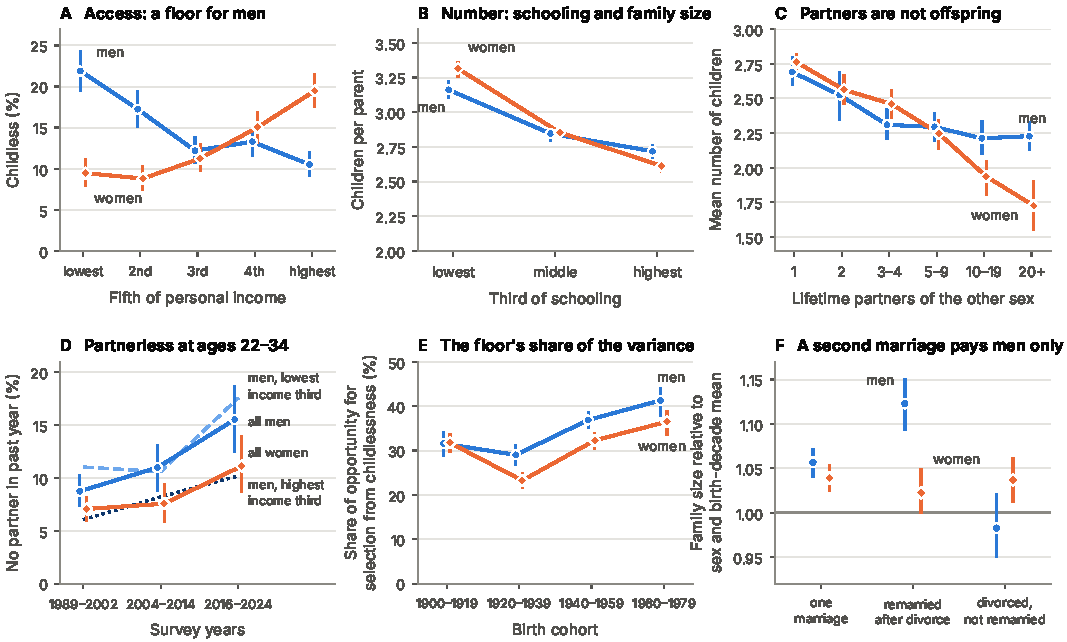
\includegraphics[width=\textwidth]{figures/fig6_today.pdf}
\caption{\textbf{Where selection sits in a present-day population.} United States, General Social Survey 1972--2024, adults aged
45--79 born 1900--1979 (panel D: ages 22--34); whiskers are 95\% bootstrap intervals; men are circles and women diamonds.
\textbf{(A)}~Percentage childless by fifth of personal income within sex and birth decade: a floor for men, and a rise at the
top for women. \textbf{(B)}~Mean number of children among parents by third of schooling. \textbf{(C)}~Mean number of children by
reported lifetime number of opposite-sex partners since age 18; the category of no partners is omitted because it contains
inconsistent reports. \textbf{(D)}~Percentage reporting no sexual partner in the past year, by period; dashed and dotted lines
are men in the lowest and highest thirds of own income, shown without intervals. \textbf{(E)}~Share of the opportunity for
selection that is due to childlessness (Eq.~\ref{eq:oppsplit}), by birth cohort. \textbf{(F)}~Family size by marital history,
relative to the mean of the respondent's sex and decade of birth. Source: authors' analysis of public
data~\cite{gss2024}.}
\label{fig:today}
\end{figure*}

\emph{The door in 70 countries.} A survey of \WdN{} people in 175 countries~\cite{kowal2025} allows a test outside the
United States, with self-ratings in place of records. Within country and sex, and holding age fixed, a standard deviation
of a man's rating of his own financial prospects goes with \WdDoorResM{} percentage points in the probability that he has
a partner (\WdDoorResMCI). For a woman the figure is \WdDoorResW{} (\WdDoorResWCI), and the difference is \WdDoorResDiff{}
points (\WdDoorResDiffCI; \WdDoorN{} people in \WdCtry{} countries with at least fifty of each sex;
Fig.~\ref{fig:world}C). Men's coefficient exceeds women's in \WdDoorCtryPos{} of the \WdDoorCtry{} countries with enough
respondents to estimate each. Looks go with having a partner in both sexes (\WdDoorLooksM{} and \WdDoorLooksW{} points).
Self-rated kindness goes with nothing (\WdDoorKindM{} and \WdDoorKindW), though kindness is what both sexes say they want
most (Section~\ref{sec:resculture}). These are cross-sectional self-reports, and having a partner may itself raise a man's
view of his prospects.

\emph{Who becomes an ancestor.} A popular reading of the genetic record holds that twice as many women as men left
descendants, or that only half of all men ever fathered a child~\cite{baumeister2010}. The observation behind it is sound.
Mitochondrial lineages coalesce about twice as deep as Y-chromosome lineages in each of three
populations~\cite{wilder2004}, and comparisons of maternal, paternal and X-linked diversity point the same
way~\cite{hammer2008,lippold2014}. The reading is not. Such data estimate a ratio of effective numbers, and for a sex in
which a share $q$ leaves no offspring and family size among the rest has mean $m$ and variance $m+\alpha m^2$,
\begin{equation}
\frac{N_e}{N}=\frac{1-q}{1+\alpha}\label{eq:ancestors}
\end{equation}
whatever the mean (Proposition~\ref{prop:ancestors}; simulation within \NtAncErr\%). A twofold ratio follows if 80\% of
women and 40\% of men reproduce and parents of each sex are otherwise alike. It follows equally if the same share of each
sex reproduces and fathers differ among themselves as much as $\alpha=1$ implies, as under polygyny, and competition among
patrilineal clans produces it with no difference in headcounts at all~\cite{zeng2018,karmin2015}
(Fig.~\ref{fig:choice}D). Nor does a lineage hold twice as much female DNA: mother and father contribute equally to every
child's other chromosomes. In the United States the two effective numbers are nearly equal, \VgNeM{} of the census number
for men and \VgNeW{} for women born 1900--1979, a ratio of \VgNeRatio{} (\VgNeRatioCI). The ratio has risen to
\VgNeRatioNew{} (\VgNeRatioNewCI) among those born 1960--1979, as men's childlessness reached \VgQMNew\% against women's
\VgQWNew\%. What the genetic ratio does establish is that men's reproduction was the more unequal for a very long time.
That is the condition under which a floor at the door selects: excluding 40\% of men puts an intensity of \NtIqForty{}
standard deviations on whatever admits the rest (Corollary~\ref{cor:floor}); the \VgQM\% excluded in the United States
puts \NtIqUS.

\subsection{A jury chose, and the bride was often not asked}\label{sec:reschoice}

\begin{figure*}[t]
\centering
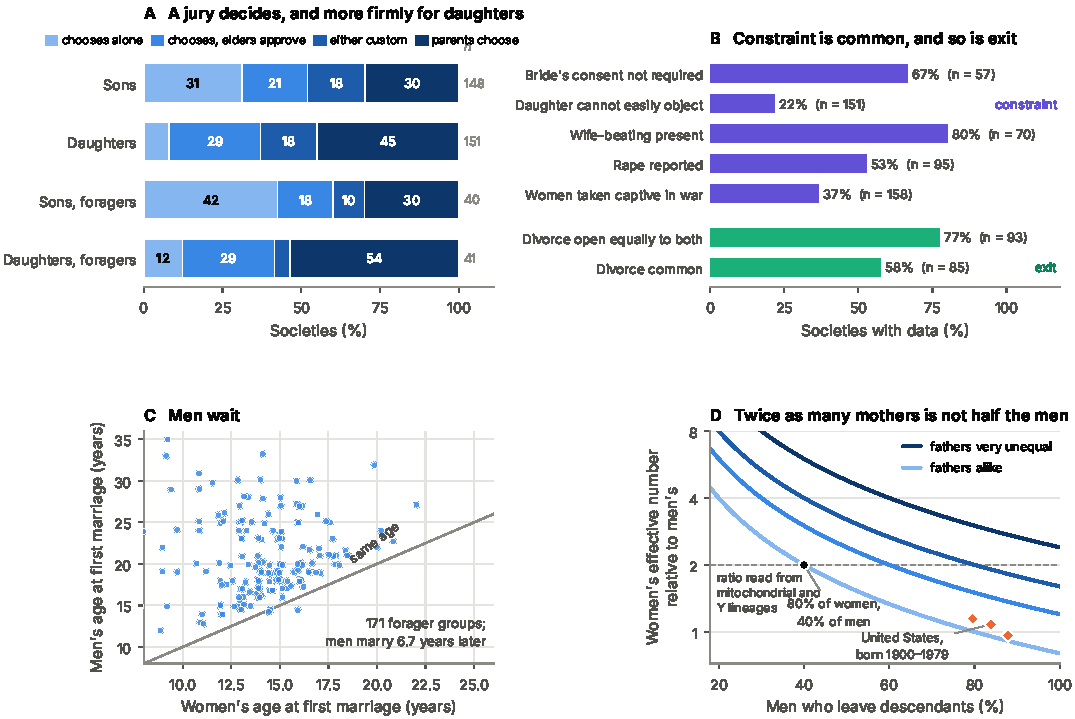
\includegraphics[width=\textwidth]{figures/fig7_choice.pdf}
\caption{\textbf{Who decided, and who became an ancestor.} \textbf{(A)}~Who chooses a spouse, for sons and for daughters, in
the Standard Cross-Cultural Sample and among its foragers (codes of Broude and Greene~\cite{broude1983}; numbers of societies
at right). \textbf{(B)}~Percentage of societies with data in which each practice is coded: constraint on the bride and
coercion (violet), and exit from marriage (green)~\cite{frayser1985,broude1983,sanday1981book,white1988,whyte1978}.
\textbf{(C)}~Age at first marriage of men against women in \CcAgeN{} hunter-gatherer groups~\cite{binford2001}.
\textbf{(D)}~Ratio of women's to men's effective number against the share of men who leave descendants, when 80\% of women
do, for four degrees of inequality among fathers ($\alpha=0$, 0.5, 1, 2; Eq.~\ref{eq:ancestors}). Dashed line: the twofold
ratio read from uniparental lineages~\cite{wilder2004}; circle: the popular reading of it; diamonds: three United States
birth cohorts. Sources: authors' analysis of the D-PLACE release~\cite{kirby2016} and of public survey data~\cite{gss2024}.}
\label{fig:choice}
\end{figure*}

The words mate choice suggest a young woman choosing freely. The coded ethnographic record says otherwise
(Fig.~\ref{fig:choice}A,B; Table~\ref{tab:cultures}). In the Standard Cross-Cultural Sample of \CcSccsN{}
societies~\cite{murdock1969,kirby2016} a daughter chooses her husband alone in \CcAloneW\% of \CcArrWomenN{} societies, and a
son his wife in \CcAloneM\% of \CcArrMenN. Parents choose for \CcParW\% of daughters, and in \CcNoObjW{} societies she cannot
easily object~\cite{broude1983}. Where both sexes are coded the daughter is less free than the son in \CcPairDau{}
societies and freer in \CcPairSon. Foragers are no exception (parents choose in \CcParWFor\% of \CcForArrN), as an
independent coding of 190 foraging societies also found~\cite{apostolou2007,walker2011}. The bride's consent is necessary
in \CcConsNec\% of \CcConsN{} societies with information, and in \CcConsNot\% she is not consulted~\cite{frayser1985}.
Coercion is coded often where it is coded at all. Rape is reported in \CcSanPres{} of \CcSanN{}
societies~\cite{sanday1981,sanday1981book} and rated common in \CcRapeCom{} of \CcRapeN~\cite{broude1976}; women were taken
captive in war in \CcCapPct\% of \CcCapN~\cite{white1988}; wife-beating is present in \CcBeatPct\% of \CcBeatN. These codes
are ethnographers' judgments of societies described in the last two centuries. The small samples select for societies in
which the matter was recorded, and none measures the share of conceptions that followed coercion. That share, the $\kappa$
of Eq.~\eqref{eq:coercion}, is unknown for any ancestral population, and we do not guess it.

Three things follow for the hypothesis. It never needed a free bride. It needs an assessor who has watched the candidate
for years, and the record puts parents, elders and in-laws in that seat; a literature built on female choice has
underweighted them~\cite{apostolou2007,apostolou2010}. Parents weigh signs of investment and of cooperation with the family more, and signs of heritable quality such as looks
less, than their children do~\cite{buunk2008}, so their verdict loads on what long observation reveals. Second, coercion
is not outside the model. It is the contest of force of Section~\ref{sec:rescontest}, and where it decides a mating it
selects the body and the coalition in place of the mind. Third, the bride's own judgment was exercised after the wedding
more than before it. Divorce is open equally to both spouses in \CcDivEqPct\% of \CcDivN{} societies and is common in
\CcDivCommonPct\% of \CcDivFreqN~\cite{whyte1978,broude1983}. A wife who could not refuse could often leave, and leaving is
a judgment of delivery, the half that display cannot show (Section~\ref{sec:resverify}). Men, for their part, wait. In
\CcAgeN{} forager groups men first marry at \CcAgeM{} years and women at \CcAgeW, a gap of \CcGap{} years (\CcGapCI) that
is wider where more men have several wives ($r=\CcGapPolyR$; \CcGapPolyCI)~\cite{binford2001} (Fig.~\ref{fig:choice}C).
The wait falls in the years when a hunter's returns are still climbing, so a man is judged on a longer public record than
a woman is. A girl married at fourteen cannot have been chosen on a record of her own, which is one reason her assessment
continues afterward.

\subsection{Culture changes the weights, not the links}\label{sec:resculture}

The five links are found wherever they have been looked for. What varies among societies is who fills each role and how
much each kind of evidence weighs (Table~\ref{tab:culture}). Two data sets and three patterns bear on the argument.

\begin{figure*}[t]
\centering
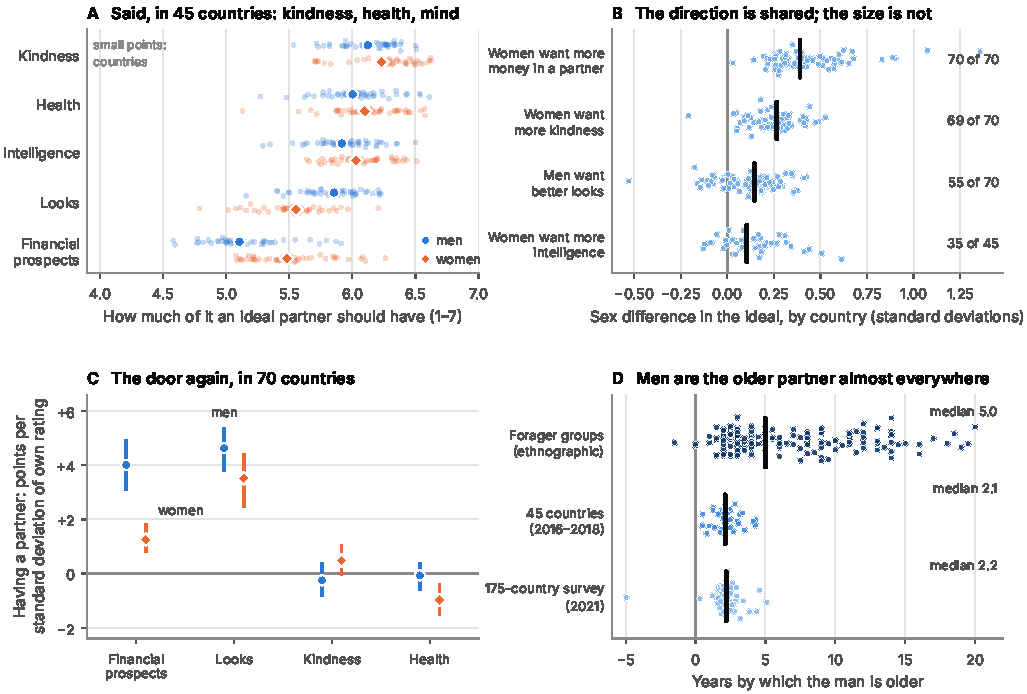
\includegraphics[width=\textwidth]{figures/fig8_world.pdf}
\caption{\textbf{The direction is shared; the size is cultural.} \textbf{(A)}~How much of each quality an ideal long-term
partner should have, in 45 countries (large markers: all respondents; small points: country means)~\cite{walter2020}.
\textbf{(B)}~Sex difference in the ideal, one point per country, in pooled standard deviations, signed so that the commonly
reported direction is positive; bar: median; right: countries with that direction. Intelligence from the 45-country
file~\cite{walter2020}, the rest from the 175-country file~\cite{kowal2025}. \textbf{(C)}~Change in the probability of having
a partner per standard deviation of a person's rating of their own financial prospects, looks, kindness and health, within
country and sex and holding age fixed, with 95\% intervals from resampling countries~\cite{kowal2025}. \textbf{(D)}~Years by
which the man is the older partner: \CcAgeN{} forager groups~\cite{binford2001} and country means from the two
surveys. Countries are units of replication and none is named. Source: authors' analysis of open data.}
\label{fig:world}
\end{figure*}

\emph{Stated ideals in 45 and 175 countries.} Two open cross-national files let the claim be checked. In 45 countries
(\WtN{} people~\cite{walter2020}) both sexes say an ideal partner should above all be kind (\WtKindM{} for men and
\WtKindW{} for women, of 7), healthy, and intelligent (\WtIntM, \WtIntW); looks (\WtLooksM, \WtLooksW) and financial
prospects (\WtResM, \WtResW) come below. Women rate intelligence above both looks and money in \WtIntAboveW{} of the 45
countries and men in \WtIntAboveM{} (Fig.~\ref{fig:world}A). A good mind is what people everywhere say they want, and it
is what four minutes cannot show them (Section~\ref{sec:resjury}). That gap between the wish and the evidence is the space
this hypothesis occupies. In the larger file (\WdPeople{} people in \WdCtry{} countries with at least fifty respondents of
each sex~\cite{kowal2025}) women want better financial prospects in a partner than men do in all \WdResPos{} countries, but
the difference runs from \WdResLo{} to \WdResHi{} standard deviations (median \WdResD). Men want better looks in
\WdLooksPos, by a median of only \WdLooksD, with reversals in the rest (Fig.~\ref{fig:world}B). Given thirty points to
divide among six qualities, both sexes give the most to kindness. Across countries the difference in wanting resources is
smaller where respondents hold more equal views of the sexes (rank correlation \WdEqRes; \WdEqResCI), as one earlier study
found and another did not~\cite{zentner2012,walter2020}, while the difference in wanting looks is larger there
(\WdEqLooks; \WdEqLooksCI). The man is the older partner on average in \WdAgePos{} of \WdAgeCtry{} countries and in all
\WtAgePos{} of the smaller sample, by a median of \WdAgeGap{} years against \CcGap{} among foragers
(Fig.~\ref{fig:world}D). These are convenience samples answering questionnaires, and countries are not independent of one
another.


\emph{Who assesses varies most.} Kin arrange most marriages among foragers~\cite{walker2011}. In the United States meeting
online is now the most common way for heterosexual couples to meet, and the part played by friends and family has
shrunk~\cite{rosenfeld2019}. By Proposition~\ref{prop:staging} that is a move from unstaged evidence held by people who
know the candidate to staged evidence exchanged between strangers. Cues of capacity survive the move; evidence of delivery
does not (prediction P28).

\emph{The floor moves with the marriage system and the sex ratio.} About 85\% of societies in the anthropological record
have permitted polygyny~\cite{henrich2012}, which raises the share of men left unpaired and, by
Corollary~\ref{cor:floor}, the intensity of selection on whatever wins wives there; normative monogamy shrinks the pool of
unmarried men~\cite{henrich2012}. Among eight Makushi communities men's mating effort resembled women's where men were in
surplus and turned toward short-term relationships only where men were scarce~\cite{schacht2015}.

\emph{What counts in a partner tracks what each sex contributes locally.} Men's greater weight on youth and looks, and
women's on resources, appear across 45 countries~\cite{walter2020}, but both sexes choose partners nearer their own age
where gender equality is greater~\cite{walter2020}, and the size of the preference gap fell with gender parity in one
analysis~\cite{zentner2012} and not robustly in another~\cite{walter2020}. Where a wife's earnings cross a norm the market
registers it: the share of couples in which the wife earns just over half of household income drops
sharply~\cite{bertrand2015}, and promotion to a top job doubled the probability of divorce for women and not for men, in
traditional couples only~\cite{folke2020}. Cues are local as well: heavier bodies were preferred in poorer
sites~\cite{swami2010}, masculine faces where health was worse~\cite{debruine2010}, and the usual readings of facial
masculinity were weak or reversed in small-scale societies~\cite{scott2014}. None of this is a difference between kinds of
people. Each is a response to who pays, who watches and what is scarce.

\begin{table*}[t]
\caption{What varies among societies, and the link it moves. Each row cites a comparative study; ``moves'' names the
parameter of the models in Section~\ref{sec:theory} that the practice changes. The rows are associations across or within
societies, not experiments, and none ranks a population.}
\label{tab:culture}
\scriptsize
\begin{tabularx}{\textwidth}{@{}P{0.13\textwidth}LP{0.25\textwidth}P{0.17\textwidth}@{}}
\toprule
What varies & Evidence & Link and parameter it moves & Consequence in the model\\
\midrule
Who chooses &
Parents or kin arrange marriages in about 85\% of 190 foraging societies~\cite{walker2011,apostolou2007} and weigh investment
and cooperation more than their children do~\cite{buunk2008}; in the United States meeting online has displaced friends and
family~\cite{rosenfeld2019}. &
Link 1, who assesses; unstaged observation $(1-d)n$ and so the validity for delivery $R_p$. &
Delivery is selected where the jury knows the candidate (Proposition~\ref{prop:staging}).\\
Marriage system &
About 85\% of societies have permitted polygyny~\cite{henrich2012}; polyandry is permitted in 53 societies outside its classical area, most often egalitarian
ones~\cite{starkweather2012}; beliefs in several fathers per child are widespread among 128 lowland South American
societies~\cite{walker2010}. &
Link 4, the episode; the share of men unpaired, $q$. &
Intensity $\varphi(z_q)/(1-q)$ rises with $q$ (Corollary~\ref{cor:floor}).\\
Payments and service &
Brideservice, brideprice or exchange in about 80\% of foraging societies~\cite{walker2011}; marriage payments of four to six
times annual household income, whose direction has switched within societies~\cite{anderson2007}. &
Enforced delivery $e$ before and at marriage; which family assesses. &
Capacity is selected before commitment (Proposition~\ref{prop:enforce}).\\
Sharing norms &
Meat widely shared, much of it on demand, with ridicule and exclusion for those who
refuse~\cite{woodburn1982,peterson1993,wiessner2005}. &
Enforced delivery $e$ to the band. &
As above; standing is conferred by those who receive.\\
Sex ratio &
Men's mating effort resembles women's where men are in surplus~\cite{schacht2015}; sociosexuality tracks sex ratio across 48
nations, with sex differences in every one~\cite{schmitt2005}. &
Which sex must be accepted; the floor $q$. &
The floor falls on the more numerous sex.\\
Women's earnings and gender equality &
Partners' ages converge with gender equality~\cite{walter2020}; a drop in couples where the wife out-earns the
husband~\cite{bertrand2015}; divorce after women's promotion~\cite{folke2020}; single women understating ambition before
single men~\cite{bursztyn2017}; wives now the more schooled spouse~\cite{esteve2016}. &
Link 5, aim: the weight on a woman's capacity $b$, and what she displays. &
Display follows the audience's weights; validity for women's capacity falls where it is penalized.\\
Health and subsistence &
Heavier bodies preferred in poorer sites~\cite{swami2010}; masculine faces preferred where health is
poorer~\cite{debruine2010}; standard readings of facial masculinity weak or reversed in small-scale
societies~\cite{scott2014}; Hadza and Shuar partners valued for work and character~\cite{marlowe2004,pillsworth2008}. &
Link 2, what is observed: which cues carry weight. &
Cue validity is local (Corollary~\ref{cor:cue}).\\
Paternal investment &
Jealousy is more severe where fathers invest more and extramarital sex is rarer, across 11
populations~\cite{scelza2020}; the romantic kiss is present in 46\% of 168 cultures~\cite{jankowiak2015}. &
Mean delivery $\bar p$ and how it is policed; the form of display. &
Capacity matters in proportion to $\bar p$ (Proposition~\ref{prop:delivery}).\\
Division of labor &
Tsimane adults command a broad common repertoire~\cite{schniter2015}; occupational specialization narrows comparison to one
domain. &
Link 5, aim: the number of common domains $K$. &
Generalist aim weakens by $Kc_K$ (Proposition~\ref{prop:division}).\\
\bottomrule
\end{tabularx}
\end{table*}

\subsection{The jury is being dismissed}\label{sec:resvillage}

\begin{figure*}[t]
\centering
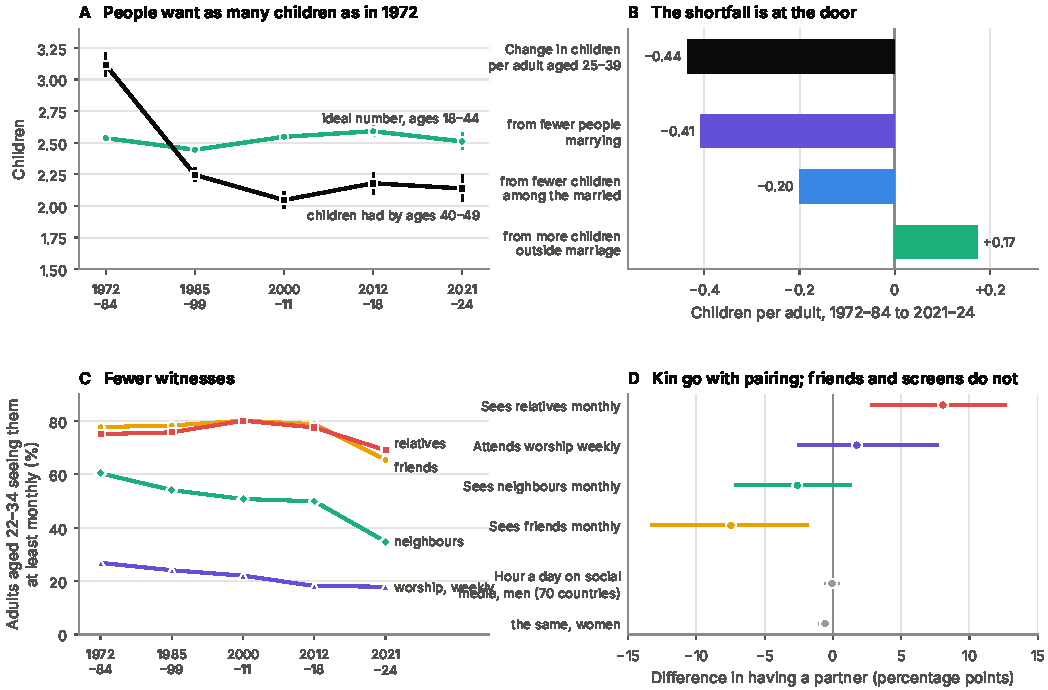
\includegraphics[width=\textwidth]{figures/fig9_village.pdf}
\caption{\textbf{Wanted, paired, born: the United States, 1972--2024.} \textbf{(A)}~Ideal number of children for a family
(adults aged 18--44) and number of children had (adults aged 40--49), by survey period, with 95\% intervals.
\textbf{(B)}~Change in children per adult aged 25--39 between 1972--1984 and 2021--2024, divided into the part due to more
people never marrying and the parts due to change within marital status. \textbf{(C)}~Adults aged 22--34 who spend a social
evening at least monthly with friends, relatives or neighbors, and who attend worship weekly. \textbf{(D)}~Difference in the
percentage with a steady partner between adults aged 22--34 who do and do not have each tie, holding age, sex, schooling,
income rank and survey year fixed; and, in grey, the difference per daily hour of social media in the 175-country
survey~\cite{kowal2025}. Associations, with 95\% bootstrap intervals. Source: authors' analysis of public
data~\cite{gss2024}.}
\label{fig:village}
\end{figure*}

If minds are read by juries over years, a society that dismisses the jury should find pairing harder. Three observations
from the United States fit that expectation, and three do not.

\emph{People want as many children as they did.} Asked the ideal number of children for a family, adults aged 18--44 said
\VgIdealOld{} in 1972--1984 and \VgIdealNew{} in 2021--2024, and those who had never married said \VgIdealNever{}
(Fig.~\ref{fig:village}A). The number people have had by their forties fell from \VgActOld{} to \VgActNew{} over the same
years. It stands at \VgActNever{} among the never married and \VgActEver{} among the ever married.

\emph{The shortfall is at the door.} Among adults aged 25--39 the number of children fell from \VgKidsOld{} to \VgKidsNew{}
per person, while the share never married rose from \VgNevOld\% to \VgNevNew\% (Fig.~\ref{fig:main}F). The move toward the
never married accounts for \VgMarr{} of the \VgChange{} (\VgMarrShare\%; \VgMarrShareCI). Change among the married
contributed \VgWithinEver, and more children outside marriage \VgWithinNever{} (Fig.~\ref{fig:village}B).
This is an accounting of where the births went and not a cause, since people who want no children may not marry. But the
stated ideals did not move. Later and less marriage runs with later and fewer births in East Asia too~\cite{raymo2015}, the
recent Nordic decline is of births forgone and not only postponed~\cite{hellstrand2021}, and no economic or policy change
since 2007 explains much of the American one~\cite{kearney2022}.

\emph{There are fewer witnesses.} Among adults aged 22--34, \VgNeighOld\% spent a social evening with a neighbor at least
monthly in 1972--1984 and \VgNeighNew\% in 2021--2024; with friends, \VgFriOld\% and \VgFriNew\%. Weekly worship fell from
\VgWorOld\% to \VgWorNew\%, and time online rose from \VgOnlineOld{} to \VgOnlineNew{} hours a week since 2000--2011
(Fig.~\ref{fig:village}C; the latest surveys were partly self-administered, which may affect these answers). The share with
no sexual partner in the past year rose from \VgNoPartOld\% to \VgNoPartNew\%, and among men from \VgNoPartMOld\% to
\VgNoPartMNew\%, as others report~\cite{ueda2020,twenge2017,lei2021}. Meeting online has displaced introduction by friends
and family as the commonest way for couples to form~\cite{rosenfeld2019}. In the terms of the model, a jury holding years
of unstaged evidence gives way to one observer holding a profile, which is all test (Proposition~\ref{prop:staging}). If a
commitment waits until a partner's delivery is known to a given reliability, the wait is inversely proportional to the
number of independent witnesses and to the unstaged share of what they saw (Proposition~\ref{prop:waiting}): \NtWaitCamp{}
periods for a camp of thirty, \NtWaitFive{} for five friends, \NtWaitOne{} for one observer alone. A fertile window is
finite, so a longer wait means fewer births.

\emph{What does not fit.} Young adults who see relatives at least monthly are more often partnered (\VgAsRel{} points;
\VgAsRelCI), but those who see friends monthly are less often partnered (\VgAsFri; \VgAsFriCI), and neighbors and worship
show nothing reliable (Fig.~\ref{fig:village}D). Kin are the jury of the ethnographic record, so the first result is the
one the theory expects; but single people have more evenings free, and one survey cannot order cause and effect. Across 70
countries an hour more a day on social media goes with \WdScrM{} points more singlehood among men (\WdScrMCI) and
\WdScrW{} among women, which is next to nothing. And in one national panel couples who met online married sooner, not
later~\cite{rosenfeld2017}. The claim that survives is narrow. Births are being lost before couples form, at the step where
evidence about a partner is thinnest and, for men, where selection on standing is strongest and rising
(Table~\ref{tab:funnel}). Specialization belongs in the same account. It lengthens training, which postpones first
births~\cite{nibhrolchain2012}. It moves people away from kin, and thinner kin networks are a leading explanation of the
transition to small families~\cite{newson2005,sear2011,colleran2020}. And it replaces common comparison on many domains with
separate ladders, the condition under which selection stops favoring the generalist (Proposition~\ref{prop:division}).
Whether generalists are the better adapted to survive is not something these data can show.

\subsection{Small brains, shrinking brains and restless minds}\label{sec:reshominins}

Neanderthals reached brain sizes like ours in communities far smaller than those of later
\Hs~\cite{prufer2014,skov2022}, so no account may depend on large networks. The present one does not: in a small community
everyone observes everyone for years, so validity can be high, while the number of candidates, and hence intensity, is
low. The prediction for such populations is a slower and noisier response, not none. The two lineages also differ in
organization more than in size: Neanderthal endocasts are elongated where ours became globular~\cite{neubauer2018}, so
volume is the wrong variable for comparing their cognition and the right one for the energetic argument, since tissue is
what costs. Small-brained species persisted while large-brained ones lived elsewhere, so no account may treat enlargement
as inevitable. \textit{H.~floresiensis} is the clearest case, and it meets the conditions under which the model expects
the least response: a small population isolated on an island~\cite{sutikna2016,brumm2016}, with few candidates to choose
among and a tight energy budget. \textit{H.~naledi} is harder, since large-brained people lived in Africa at the
time~\cite{dirks2017}. In the model, tissue follows demand only when it is functionally coupled to capacity and affordable
(Proposition~\ref{prop:tissue}); cheaper calories and shared care relax the second
condition~\cite{carmody2011,hawkes1998,burkart2014}. A model given the dates of such relaxations reproduces stasis and steps, but
that is a consistency check and not a test.

\emph{Smaller brains, more of the alleles.} Brain mass has fallen since the late Pleistocene, by more than 5\% in 50,000
years on one estimate and largely in step with body size~\cite{stibel2021,ruff1997}; whether it fell again in the last few
thousand years is disputed~\cite{desilva2021,villmoare2022}. Over the last ten thousand years in West Eurasia, meanwhile,
combinations of alleles that today predict measures of cognitive performance rose by about one standard deviation on the
scale of present variation~\cite{akbari2026}. The two are compatible. Selection through assessment acts on performance,
and performance can be had from more tissue or from better use of it. When tissue becomes dearer or its marginal return
falls, the response moves to the second route (Proposition~\ref{prop:tissue}). The pattern is selection for doing more
with less, which is what engineers obtain when a small model is trained to match a large one~\cite{hinton2015}. The
caution of the source applies: those alleles were scored in industrial societies, and what they did in a Neolithic
village is unknown.

\emph{Restless minds.} Variants of the dopamine receptor gene \textit{DRD4} that are associated with novelty seeking and
with attention-deficit diagnoses show signs of past positive selection~\cite{ding2002,williams2006} and are commoner in
populations that migrated farther~\cite{matthews2011}. Among Ariaal men in Kenya, carriers were better nourished than
non-carriers in a nomadic community and worse nourished in a settled one~\cite{eisenberg2008}. In a foraging task, adults
who screened positive for attention deficits left depleted patches sooner and earned more~\cite{barack2024}. The Ariaal
study gives no percentage advantage, and we could not trace the figure of 20\% sometimes quoted. Against a simple story of
lost advantage, alleles associated with the diagnosis have been declining in frequency since the Paleolithic, long before
farming~\cite{esteller2020}. The present framework adds one thing. A trait that helps in some domains and hurts in others
is neutral when people are compared on all of them, and it becomes a deficit in exact proportion to its mean loading on
whatever narrower set a test covers (Corollary~\ref{cor:narrow}; simulated slopes \NtNarBroad{} and \NtNarHurt). Years of
seated, sustained, solitary work are such a set. On this reading a diagnosis measures a variant against a test. It does
not show that the variant was built for the forest. For heightened smell or hearing as selected traits we found no
comparable evidence: foragers name odors far better than neighboring farmers who speak a closely related
language~\cite{majid2018}, which points to practice and not to genes.

\section{Discussion}

\subsection{What we conclude}\label{sec:conclude}

Asked as ``is intelligence attractive?'', the hypothesis has no clear answer: measured intelligence can be detected but is
not itself attractive~\cite{driebe2021}, and stated preferences predict choices weakly~\cite{todd2007,eastwick2014,eastwick2025}.
Asked link by link, it yields eight conclusions. Each is marked as measured here, derived, or conjectured.

\textbf{1. Minds are read by communities, not by suitors} (measured; derived). In 45 countries both sexes say they want
kindness and intelligence in a partner above looks and money. In four minutes neither can be read: strangers do not agree
on who has them, and choose on looks. Reading a mind dependably takes dozens of independent observers or years of
acquaintance, and shared gossip does not substitute for either.

\textbf{2. The chooser was a jury, and the bride was often not asked} (measured in the coded record). The hypothesis needs
long observation by whoever decides. It does not need romance or consent. Coercion subtracts from it in proportion to its
share and selects the body in its place.

\textbf{3. Breadth built generality} (derived). Comparing everyone on $K$ kinds of performance multiplies selection on
general ability $K$-fold relative to any specialty. Separate ladders remove the multiplier.

\textbf{4. A test shows capacity; only conduct shows delivery} (derived). Safe, repeated contests can replace dangerous
ones for the first and never for the second, which must be watched on unremarkable days or enforced by third parties.

\textbf{5. Men are selected at the door and women after it} (measured in the United States; the door also in 70
countries). The door is a floor on standing, and it has been rising for men in each cohort. Selection on women runs
through when and whether births follow.

\textbf{6. ``Half of all men never reproduced'' misreads a real asymmetry} (derived; measured). The genetic record gives a
ratio of effective numbers. It shows that men's reproduction was the more unequal, not how many men had none.

\textbf{7. Culture sets the weights, not the links} (measured in \CcSccsN{} societies and in 45 and 70 countries). Women
want resources in a partner more than men do in all \WdResPos{} countries of one survey and \WtResPos{} of 45 in the
other; the size of the difference varies forty-fold.

\textbf{8. The jury is being dismissed} (measured in one country; mechanism conjectured). Americans want the children they
wanted fifty years ago. Nearly all of the shortfall arises before a couple forms, while young adults see neighbors,
friends and congregations less and meet partners as strangers. A society that wants its births back might ask first how
people come to know each other well enough to commit.

On the brain itself the fossil record tests none of this. It leaves room for it, and smaller brains carrying more of the
alleles for performance is what selection on performance under a cost on tissue would produce (conjectured). Nine
selection drivers, four acting on men, four on women and one on both, are set out with their evidence in
Section~\ref{sec:hidden} (Table~\ref{tab:drivers}).

\subsection{What the evidence corrects}

Checked against the literature, eighteen common claims fare unevenly (Tables~\ref{tab:audit} and~\ref{tab:audittoday}). Restrained
fighting is the animal norm and not a human invention. Formal games are thousands of years old, not millions, and cannot
have caused a change that was complete long before. Body shape and facial symmetry are weak guides to fertility and
health~\cite{lidborg2025,pound2014}. Preferences do not shift toward masculine men across the cycle~\cite{wood2014,jones2018}. Of
masculine traits only strength predicts both mating and reproduction~\cite{lidborg2022}. More partners do not mean more
children. The part of the popular account that holds best is its widest: hunters, gatherers, makers, storytellers and
organizers were watched for a long time by people with a stake in judging them well.

\subsection{Is the mechanism still operating?}

In part, and not toward larger brains. The floor on men's access and the value of stable unions still operate. Marriage
gates less of reproduction than it did and selects more strongly on men's income. Timing operates with its sign reversed
for schooling. The drivers that acted through child survival contribute almost no variance where nearly all children
survive. The generalist aim has been narrowed by division of labor toward one occupation per person. Information about
ability is more abundant than ever, though nothing shows that it is used more accurately than a forager's years of direct
observation. The net effects are small beside environmental change: selection on education-linked variants is about 0.01
standard units per decade~\cite{kong2017}, test-score trends in both directions arise within
families~\cite{bratsberg2018}, and brain volumes rose across twentieth-century birth cohorts~\cite{decarli2024}. An
ancient-DNA study of 15,836 West Eurasians reports that combinations of alleles which today predict measures of cognitive
performance rose over the last ten millennia, with the caution that such effects were measured in industrialized societies
and their relation to what was adaptive in the past is unclear~\cite{akbari2026}; it does not show what was selected or
through which episode. For the foreseeable future, development, health, schooling and culture will move human cognition
far more than selection will.

\subsection{For builders of artificial minds}\label{sec:ai}

Nothing in the propositions is specific to genes. They describe any population of learners that is selected, or trained,
on a score, and nine of them bear on open problems in the evaluation of artificial systems. \emph{The score sets the aim,
not the pressure.} More intense selection on one score yields more of whatever the score loads on
(Proposition~\ref{prop:aim}); if reward is enough to produce intelligence~\cite{silver2021}, what is rewarded decides which
intelligence. \emph{Breadth selects generality.} Averaging over $K$ tasks that every candidate must attempt multiplies
selection on what the tasks share by $K$ (Eq.~\ref{eq:mainaim}), the formal case for ability-oriented over task-oriented
evaluation~\cite{hernandezorallo2017,legg2007}; a leaderboard on which each system is ranked on its best task restores the
specialist (Proposition~\ref{prop:division}), a single benchmark invites shortcuts~\cite{geirhos2020}, and aggregate scores
hide them~\cite{burnell2023}. \emph{Judges that share their errors agree without being right.} Independent evaluators add
accuracy as Eq.~\eqref{eq:sb} says; evaluators with a common source of error, such as one rubric or one body of training
data, add agreement and stop at the ceiling of Eq.~\eqref{eq:ceiling}, so agreement among judges does not measure their
accuracy. \emph{Breadth taxes gaming, except gaming that generalizes} (Corollary~\ref{cor:inflation}):
an indicator on which decisions depend comes under pressure~\cite{campbell1979}, and only evidence of a different kind
removes a general talent for passing tests. \emph{A recognized test measures capability, not disposition}
(Proposition~\ref{prop:staging}): an evaluation that a system can tell from use bounds what it can do and says nothing
about what it will do, so disposition has to be observed in use or made not to matter by limits on what the system can
reach (Proposition~\ref{prop:enforce}), the argument of a companion manuscript~\cite{taylor2026iina}. \emph{What is enforced
is no longer selected.} In the same proposition, guaranteeing an outcome removes the pressure that would have produced the
disposition to deliver it. \emph{A narrow test makes a deficit of a difference.} A system that trades strength on some
tasks for strength on others is neutral on a broad suite and fails a benchmark confined to its weak side
(Corollary~\ref{cor:narrow}); what a benchmark calls a defect may be a property of the benchmark. \emph{A price on size
selects efficiency.} Score selection with a cost on parameters moves gains from scale to use, as it appears to have done
in our own lineage and as distillation does by design~\cite{hinton2015}. \emph{A safe test can replace a dangerous one
only for capability} (Eq.~\ref{eq:ritual}): sandboxed trials, repeated, read what a system can do and say nothing of what
it will do when the stakes are real. These are parallels of form. They are not evidence about any system.

\subsection{Relation to other accounts}

The mechanism is an amplifier on the demand side. It does not replace ecological, social or cultural
accounts~\cite{kaplan2000,gonzalezforero2018,dunbar1998,muthukrishna2018}, which say why capacity is useful; it specifies a
channel through which usefulness could become persistent selection, and it makes predictions they do not: that breadth of
common comparison matters more than depth of culture, that the criterion of standing matters more than the intensity of
competition, that a preference cannot outrun the instrument that serves it, and that selection weakens where access is
decoupled from assessed performance. It does not explain the energy budget or the developmental supply of variants.

\subsection{Limitations}

No ancestral parameter is estimated. The models are Gaussian and mostly one-generation. Deception enters only in its
simplest form, delivery conditional on being assessed (Proposition~\ref{prop:staging}); display and assessment do not
coevolve, and enforcement is given, not derived. A product of correlations cannot show that the channel operated, and we
make no such claim (Section~\ref{sec:strength}). Phenotypic validity is not genetic accuracy. The generalist results assume
independent, equally weighted domains. The speed-dating sample is graduate students at one university, selected for
academic ability, in a setting that is all test; the law of Eq.~\eqref{eq:sb} should travel, the particular agreements
need not. The survey analysis is phenotypic and from one country, and its access component includes chosen childlessness
and infertility. The cross-cultural rows are associations. The ethnographic codes are outsiders' judgments of recently described societies, the cross-national files are convenience samples of self-report, and the division of falling births is an accounting and not a cause. Claims were checked against abstracts, not full texts. A
register of \NObj{} objections and the conditions under which the pathway fails are in Sections~\ref{sec:redteam}
and~\ref{sec:limits}.

\subsection{What would count against it}

Section~\ref{sec:predictions} lists \NPred{} predictions with the results that would weaken each. Seven are decisive.
Diverse observation should beat repeated observation of one domain at fixed total time (P2). Standing should track
independently measured general capacity where it is conferred as prestige and not where it is taken by force (P5, P13). In
natural-fertility populations selection on men's standing should lie in access at the low tail and not in family size among
fathers (P17). A person competent in several domains should be judged higher in general ability, and preferred as a
long-term partner or ally, over a specialist of equal total excellence (P22). Evidence of reliable investment should
raise the weight of competence in consequential choices (P23). Judgments of reliability formed from unannounced
observation should predict later conduct better than judgments formed from the same amount of staged interaction, with the
reverse for ability (P24). And lengthening an encounter or adding observers should shift the weight of choice toward
intelligence and sincerity (P27). If these fail, the mechanism fails with them.

\section{Methods}\label{sec:methods}

\emph{Fossil record.} Three open compilations were used as published: 233 crania with consensus dates and
volumes~\cite{gingerich2022}, 166 \Homo{} specimens with taxon, age and site~\cite{will2021}, and 94 early
hominins~\cite{du2018}. Piecewise-linear models of log volume on time were compared by AICc and BIC; change points were
located by grid search with \FosBoot{} bootstrap resamples. Regional series were assigned by site coordinates
(Section~\ref{sec:explananda}).

\emph{Theory and simulation.} The nineteen propositions are derived for Gaussian traits under additive inheritance
(Section~\ref{sec:theory}); proofs are in Section~\ref{app:proofs}. Each was checked by Monte Carlo or individual-based
simulation against its exact value, and re-derived by an independent construction that shares no code with the experiments
(Section~\ref{sec:experiments}). Parameter values are illustrations, not estimates.

\emph{Speed dating.} The public file of the Columbia experiment~\cite{fisman2006} has \SdRows{} rows, one per person per
meeting, for \SdN{} people. Ratings are on a 1--10 scale and were
centered on each rater's mean. Agreement between two observers is the one-way intraclass correlation among the ratings a
person received; agreement between panels is the correlation, across persons, of the means of two disjoint random sets of
$k$ raters. What predicted a yes is a linear probability model of the decision on the six ratings,
standardized over all meetings, with a fixed effect for each chooser, fitted separately by sex, using either the chooser's
own ratings or the mean rating the partner received from everyone else. Expected interest is the 1--10 guess that the
partner would say yes, rescaled to 0--1. Intervals are percentile bootstraps over persons. Variables describing race and
religion were not used (Section~\ref{sec:speed}).

\emph{Present-day selection.} The General Social Survey cumulative file, 1972--2024~\cite{gss2024}, supplied \GssN{} respondents
aged 45--79 born 1900--1979 with known number of children. Traits were years of schooling, a ten-word vocabulary test,
occupational prestige, and the logarithm of personal income at ages 45--64. Each trait was standardized, and fitness made
relative, within sex and decade of birth; cells were combined by their weights. Access, number, pairing and conversion
follow Eq.~\eqref{eq:split}. Survey weights were applied. Intervals are percentile bootstraps (\GssBoot{} resamples of
respondents within cells; 500 to 1,000 for the later analyses). Results were stable without weights, in the age window
50--74, and in surveys before and after 1990 (Section~\ref{sec:sitables}). Only aggregates by sex and cohort are reported.

\emph{Ethnographic codes.} We used the D-PLACE release~\cite{kirby2016} of the Standard Cross-Cultural
Sample~\cite{murdock1969} (\CcSccsN{} societies), of the Ethnographic Atlas (\CcEaN) and of Binford's hunter-gatherer
compilation~\cite{binford2001} (\CcBinN{} groups): who chooses a spouse, and wife-beating~\cite{broude1983};
consent~\cite{frayser1985}; rape~\cite{broude1976,sanday1981book}; captives~\cite{white1988}; divorce~\cite{whyte1978}; ages at
first marriage and polygyny~\cite{binford2001}; games~\cite{roberts1959}. Foragers are societies whose dominant subsistence is
gathering, hunting or fishing. Missing codes were dropped variable by variable. Societies share ancestry and neighbors, so
we give counts and shares and claim no significance across them; the interval for the forager age gap resamples groups and
ignores their relatedness. For games we report presence only (Section~\ref{sec:notes}).

\emph{Cross-national surveys.} The 175-country file~\cite{kowal2025} (\WdN{} rows) and the 45-country
file~\cite{walter2020} (\WtN{} rows) were read as deposited. A country enters a country-level analysis if it has at least
fifty men and fifty women with the variable (thirty in the smaller file). Sex differences are differences in pooled
standard deviations. Having a partner was regressed on four self-ratings standardized within country and sex, with age and
its square, after removing country means; intervals resample countries. No country is named or ranked.

\emph{Births, ideals and ties.} A second extract of the General Social Survey supplied marital status, number of
children, ideal number of children, social evenings, worship, hours online and partners in the past year. The change in
children per adult aged 25--39 was divided, by the standard decomposition of a difference between two rates, into a part
due to the share never married and parts due to change within marital status. Effective numbers use
$N_e/N=\bar k/(\bar k-1+V/\bar k)$ on completed families, which equals Eq.~\eqref{eq:ancestors} identically. Ties were
related to having a steady partner by a linear probability model with age, sex, schooling, income rank and year.

\emph{Literature.} Searches ran to November 10, 2026. Of \RefCited{} references, \RefResolved{} have a DOI resolved
against Crossref; specific claims were checked against abstracts where one could be retrieved, and otherwise limited to
what the title states.

\section*{Data and code availability}

\noindent All code, results and the three fossil datasets are in the accompanying package; one script rebuilds every number,
table and figure. The survey file and the speed-dating file are public and are downloaded by scripts that verify them, not
redistributed (Section~\ref{app:repro}).
